\documentclass{article}

\usepackage[utf8]{inputenc}
\usepackage[T1]{fontenc}
\usepackage{textcomp}
\usepackage[italian]{babel}
\usepackage{graphicx}
\usepackage{siunitx}
\usepackage{hyperref}
\usepackage{float}
\usepackage{amsmath, amssymb}

\sisetup{uncertainty-mode=separate}

\title{Relazione di Laboratorio 1 - Pendolo Quadrifilare}
\author{Iallorenzi Michele - Wallout Francesco}

\begin{document}

\maketitle

\section{Introduzione}
    L'esperimento verte sullo studio del moto del Pendolo Quadrifilare al fine di dimostrare la validità della relazione predetta dalla teoria tra il periodo e l'ampiezza dell'angolo di oscillazione del pendolo. 
    Per studiare questo fenomeno, "usciamo" dal regime delle piccole oscillazioni e posizioniamo il pendolo in modo da avere un moto più duraturo (nel tempo), con ampie oscillazioni.
    Il pendolo è composto da 4 fili che sorreggono un pezzo di legno (agli spigoli del blocco), in questo modo la traiettoria del pendolo si sviluppa su un piano (avviene un moto piano) ed il pendolo sarà stabile.\\
    Al di sotto del blocchetto, troviamo un pezzo di piombo, che serve ad aumentare il peso dell'oggetto e rendere quindi trascurabile l'attrito dell'aria ed altre possibili perturbazioni.\\
    Una bandiera metallica attaccata al pendolo ottura una fotocellula ogni volta
    che il pendolo raggiunge il punto più basso della sua traiettoria, questo permette
    ad un calcolatore connesso alla fotocellula di misurare il periodo di otturazione e il
    tempo di transito, ovvero il tempo per cui la fotocellula rimane coperta in ciascun
    passaggio.
    
\section{Esperienza}

    \subsection{Strumenti}
    \begin{itemize}
        \item Pendolo Quadrifilare
        \item Cronometro
        \item Fotocellula (per contare le oscillazioni e la velocità istantanea)
    \end{itemize}
    
    \subsection{Misurazione}
    Posizionare il grave ad un ampiezza abbastanza grande per permettere al pendolo di oscillare il più a lungo possibile. Appena parte il moto del pendolo, bisogna far partire il cronometro e poi fermarlo quando la bandiera del pendolo non registra più nessun oscillazione.
    Prima di questo esperimento è necessario prendere queste misure: "lunghezza del filo" (distanza tra punto di sospensione e centro di massa) ($l$), larghezza della bandierina ($w$), distanza tra punto di sospensione ed estremo della bandierina ($d$).
    
    
\section{Elaborazione dati}

    \subsection{Velocità del Pendolo}
    Sappiamo che la velocità di un qualsiasi pendolo (reale) diminuisce nel tempo. Immaginiamo quindi che ci sia uno smorzamento della velocità che varia sicuramente nel tempo, ma come varia la funzione velocità in funzione del tempo? 
    Per scoprirlo facciamo un grafico che rappresenti le velocità in funzione del tempo e per ottenere la velocità del pendolo utilizziamo questa relazione:
    \begin{equation}\label{eq:velocità}
        v = \frac{w l}{t_T d}
    \end{equation}
    ($t_T$ è il tempo di transito della bandierina nel punto di massima velocità)
    Otterremo il grafico in figura \ref{fig:pendolo_quadrifilare_velocità}.\\
    \begin{figure}[ht!]
        \centering
        \includegraphics[width=0.8\textwidth]{extra/pendolo_quadrifilare_velocità.pdf}
        \caption{Grafico delle velocità massime di ciascun oscillazione in funzione del
        tempo trascorso.}
        \label{fig:pendolo_quadrifilare_velocità}
    \end{figure}
    Grazie alla scala semilogaritmica, notiamo subito che i dati sembrano disporsi approssimativamente secondo una legge esponenziale, quindi cerchiamo una relazione che sarà del tipo:
    \begin{equation}
            v(t) = v_0 e^{-\lambda t}
    \end{equation}
    Come valore per il parametro $v_0$ utilizziamo semplicemente il primo valore ottenuto tramite l'equazione \ref{eq:velocità}.
    Per trovare il valore $\lambda$ eseguiamo un fit dei minimi quadrati utilizzando
    la funzione curve\_fit di scipy, in questo modo troveremo un certo valore di $\lambda$,
    da cui possiamo inoltre ottenere il tempo di smorzamento $\tau = \frac{1}{\lambda}$.\\
    Il fit ottenuto è mostrato in figura \ref{fig:pendolo_quadrifilare_velocità}.
    \begin{gather*}
        v_0 = \SI{0.740 \pm 0.002}{\m\per\s} \\
        \lambda = \SI{0.0020468 \pm 0.0000009}{\Hz}  \\
        \tau \pm \sigma_{\tau}= \frac{1}{\lambda}\pm \frac{\sigma_{\lambda}}{\lambda^2}=\\
        =\SI{488.5\pm 0.2}{\s}
    \end{gather*}



    \subsection{Periodo del pendolo}
    Per calcolare l'ampiezza delle oscillazioni, assumiamo trascurabile l'attrito con l'aria e ricaviamoci la relazione energetica:
    \begin{equation}
        mgl(1-cos\theta_0) = \frac{1}{2}m v_0^2
    \end{equation}
    ottenuta uguagliando l'Energia Potenziale nel punto di massima altezza e l'Energia Cinetica nel punto di massima velocità per il Teorema della Conservazione dell'Energia Meccanica (ovviamente le forze in gioco sono tutte conservative e quelle non conservative fanno lavoro nullo). Si ricava che:
    \begin{equation}\label{eq:ampiezza}
        \theta_0 = \arccos\left(1 -\frac{v_0^2}{2gl}\right)
    \end{equation}
    Sappiamo che è possibile fare uno sviluppo in serie di Taylor del periodo del pendolo, ottenendo il seguente risultato:
    \begin{equation}\label{eq:T}
        T = 2 \pi \sqrt{\frac{l}{g}}\left(1 + \frac{1}{16}\theta_0^2 + \frac{11}{3072}\theta_0^4 + ...\right)
    \end{equation}
    Nel codice e nelle formule useremo solamente il secondo ordine di questo sviluppo e verificheremo
    quindi la validità di questa approssimazione.\\
    L'angolo $\theta$ è noto perché si ottiene dalla \ref{eq:ampiezza}, che varia secondo la velocità e quest'ultima è nota per la \ref{eq:velocità}.\\
    Possiamo inoltre ottenere un incertezza $\sigma_T$ per i periodi predetti
    da questo modello attraverso la normale propagazione delle incertezze, conoscendo le
    incertezze di misura su $l$, $d$ e $w$; risulta che il valore massimo di $\sigma_T$ è $\SI{0.03}{\s}$\\
    Abbiamo quindi sovrapposto i grafici delle misure di $T$ ottenute in laboratorio e di
    quelle previste dalla \ref{eq:T}, il risultato è mostrato in figura \ref{fig:pendolo_quadrifilare_periodo}
    \begin{figure}[ht!]
        \centering
        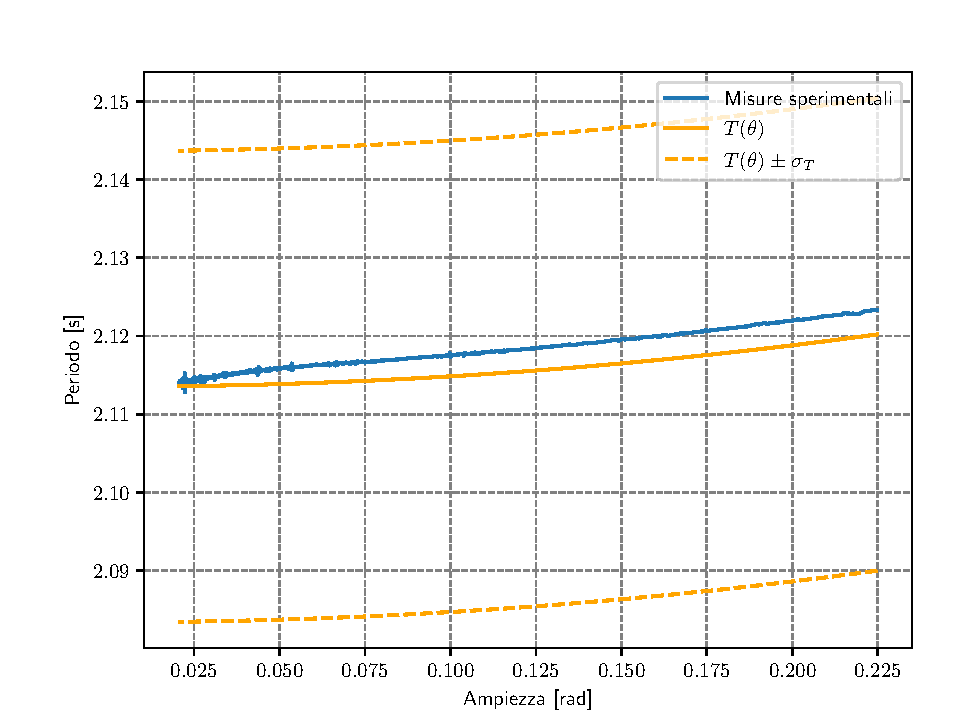
\includegraphics[width=0.8\textwidth]{extra/pendolo_quadrifilare_periodo.pdf}
        \caption{Grafici dei valori di $T$ previsti dalla teoria e misurati in laboratiorio}
        \label{fig:pendolo_quadrifilare_periodo}
    \end{figure}
    \section{Conclusioni}
    Il fit ottenuto mostrato in figura \ref{fig:pendolo_quadrifilare_velocità} si dimostra
    insoddisfacente dato l'elevato valore del $\chi^2$, possiamo quindi affermare che
    lo smorzamento del pendolo, almeno sul lungo periodo analizzato, non segue un modello
    esponenziale e che quindi i valori ottenuti per $\lambda$ e $\tau$ non sono fisicamente
    sensati.\\
    Per quanto riguarda i periodi in funzione delle ampiezze, invece, il grafico 
    \ref{fig:pendolo_quadrifilare_periodo} mostra come il modello matematico è molto
    vicino ai valori sperimentali relativamente all'incertezza di misura.

\end{document}
